\clearpage
\section{Nhiệm vụ 1 -- VG150: dự đoán quan hệ và tri thức nền}
\subsection{Thiết lập PredCls và mô hình}
Đầu vào là ảnh, hộp và nhãn object GT; đầu ra là predicate cho cặp object có
hướng. Không dự đoán lại object và không đưa cạnh quan hệ GT vào graph message
passing. VG150 là tập con của Visual Genome~\cite{krishna2017visualgenome}.

\begin{table}[H]\centering\small
\caption{Thiết lập thực nghiệm VG150.}\label{tab:vgsetup}
\begin{tabularx}{\linewidth}{@{}p{40mm}X@{}}\toprule
Thành phần & Cấu hình\\\midrule
Split, vocabulary & Train 57.723 / val 5.000 / test 26.446 ảnh; 150 object, 50 predicate và background.\\
Đặc trưng object & CLIP ViT-B/32 đóng băng, 512 chiều; hình học 5 chiều; label embedding học được 32 chiều.\\
MLP / GAT & MLP phân lớp cặp, không message passing; GAT 2 lớp, 4 heads, hidden 256, dropout 0,1.\\
Graph đầu vào & Cạnh có hướng giữa các object; edges-off bỏ cạnh giữa các object, vẫn giữ self-loop.\\
KG & Embedding 64 chiều và bit liên kết hợp lệ; WordNet 150/150, ConceptNet 138/150 lớp object.\\
Tối ưu & AdamW, learning rate $10^{-3}$, weight decay $10^{-2}$; effective batch 512, negative ratio 3.\\
Dừng và seed & Tối đa 200 epoch, patience 15; seed 42, 123, 3407. Giữ checkpoint đã chọn từ validation.\\
Đánh giá cuối & 18 cấu hình $\times$ 3 seed = 54 checkpoint; inference batch 128, cùng test và evaluator reference-v1.\\
\bottomrule\end{tabularx}\end{table}

Với object $i$, đặc trưng là $x_i=[v_i;b_i;e(c_i);k_i;m_i]$,
trong đó $k_i$ và $m_i$ chỉ có ở nhánh KG. GAT~\cite{velickovic2018gat} tính
\[
h_i^{(\ell+1)}=\mathop{\Vert}_{a=1}^{H}
\sigma\!\left(\sum_{j\in\mathcal N(i)}\alpha_{ij}^{(\ell,a)}
W^{(\ell,a)}h_j^{(\ell)}\right),\qquad
z_{ij}=f_\theta(h_i,h_j,\text{đặc trưng cặp}).
\]
MLP không tổng hợp hàng xóm. KG lấy từ
WordNet/ConceptNet~\cite{miller1995wordnet,speer2017conceptnet}, nhúng bằng
TransE, RotatE hoặc ComplEx~\cite{bordes2013transe,sun2019rotate,trouillon2016complex};
không lấy quan hệ test để xây KG.

\subsection{Protocol và kiểm soát so sánh}
Reference-v1 khớp đúng predicate, lớp subject/object và IoU của cả hai hộp
ít nhất 0,5. R@K là trung bình recall theo ảnh; mR@K tính recall theo ảnh
cho từng predicate rồi trung bình trên 50 lớp. GT trùng được giữ khi chấm.
Trong train, sampler bỏ cặp có nhiều predicate khác nhau; cần lưu ý khác biệt
giữa supervision huấn luyện và GT đánh giá khi đọc lỗi đa nhãn.

Hai đợt inference gồm 27 checkpoint gốc và 27 checkpoint loss/fusion.
Checkpoint và source được khóa, không chọn lại theo test hay evaluator mới.
Các thiết kế cải tiến dựa trên train/validation. Test đã từng được dùng ở các
vòng trước nên không mô tả đây là holdout chưa từng xem; cũng không suy từ
thứ tự thời gian rằng thiết kế loss đã được tinh chỉnh theo test.
\srcnote{Nguồn: \texttt{docs/evaluation/PredCls.md};
\texttt{reports/level1/reference-test27-v1/} và
\texttt{reference-loss-fusion-test27-v1/}.}

\clearpage
\subsection{MLP, GAT và KG: bảng test chính}
\begin{table}[H]\centering\small
\caption{VG150 test, GC reference-v1; mean $\pm$ sample std (\%), ba seed.}\label{tab:vgmain}
\begin{tabular}{@{}lrrrr@{}}\toprule
Cấu hình & R@50 & R@100 & mR@50 & mR@100\\\midrule
MLP & $63,56\pm0,77$ & $66,40\pm0,29$ & $16,95\pm1,52$ & $19,52\pm1,42$\\
GAT & $63,87\pm0,73$ & $66,21\pm0,70$ & $\mathbf{18,61\pm0,25}$ & $\mathbf{20,95\pm0,21}$\\
KG-off & $63,89\pm0,38$ & $66,24\pm0,30$ & $18,44\pm0,29$ & $20,72\pm0,43$\\
WordNet--TransE & $64,15\pm0,29$ & $66,69\pm0,34$ & $17,84\pm0,09$ & $20,34\pm0,08$\\
WordNet edges-off & $64,11\pm1,15$ & $66,46\pm1,13$ & $18,41\pm0,90$ & $20,72\pm0,76$\\
ConceptNet--TransE & $64,10\pm0,27$ & $66,45\pm0,28$ & $18,39\pm0,29$ & $20,71\pm0,28$\\
ConceptNet edges-off & $\mathbf{64,59\pm0,19}$ & $\mathbf{66,97\pm0,16}$ & $18,15\pm0,28$ & $20,47\pm0,32$\\
ConceptNet--RotatE & $64,21\pm0,37$ & $66,60\pm0,46$ & $18,57\pm0,42$ & $20,93\pm0,35$\\
ConceptNet--ComplEx & $64,37\pm0,18$ & $66,79\pm0,25$ & $18,33\pm0,24$ & $20,75\pm0,18$\\
\bottomrule\end{tabular}\end{table}

GAT tăng \textbf{1,65 pp mR@50} so với MLP, cùng dấu ở cả ba seed
($+0,970/+3,131/+0,861$ pp). Tuy nhiên R@100 giảm 0,19 pp.
Các nhánh ghép KG tại node chưa vượt GAT về mean mR@50.
WordNet--TransE thấp hơn KG-off 0,60 pp; RotatE gần GAT ($-0,04$ pp),
với một seed giảm.

Edges-off ở WordNet và ConceptNet cho R cao hơn hoặc gần bản có cạnh:
message passing không có lợi ở mọi nhánh. GAT và KG-off là các cấu hình/checkpoint
riêng; không coi các hàng là một checkpoint bật/tắt lúc inference.

\subsection{Adjusted loss: tác động lớn hơn KG}
Dùng prior $p_c$ tính từ train với add-one smoothing:
\[
\mathcal L_{\mathrm{adj}}
=\operatorname{CE}\!\left(z+\tau\log p_{\mathrm{train}},y\right),
\qquad \tau=0,25.
\]
Phần cộng prior chỉ áp dụng khi train; inference dùng logits gốc $z$.
Bốn cấu hình tạo đối chứng chéo giữa loss và KG.

\begin{table}[H]\centering\small
\caption{Loss ablation trên VG150 test. Baseline riêng, không trộn với bảng~\ref{tab:vgmain}.}\label{tab:loss}
\begin{tabular}{@{}lrrrr@{}}\toprule
Cấu hình & R@50 & R@100 & mR@50 & mR@100\\\midrule
CE, KG-off & $64,42\pm0,10$ & $66,85\pm0,09$ & $18,11\pm0,16$ & $20,56\pm0,19$\\
CE, KG-on & $63,63\pm0,14$ & $65,93\pm0,13$ & $19,27\pm0,75$ & $21,51\pm0,91$\\
Adjusted, KG-off & $62,18\pm0,16$ & $64,81\pm0,13$ & $24,59\pm0,93$ & $27,89\pm1,02$\\
Adjusted, KG-on & $62,01\pm0,31$ & $64,71\pm0,46$ & $24,67\pm1,07$ & $28,00\pm1,19$\\
\bottomrule\end{tabular}\end{table}

Giữ KG-off, adjusted tăng \textbf{6,48 pp mR@50} nhưng giảm
\textbf{2,24 pp R@50}. Với KG-on, mR tăng 5,40 pp.
Thêm KG vào adjusted chỉ tăng 0,09 pp mR@50 và có seed giảm 2,09 pp:
lợi ích chính đến từ loss, chưa có bằng chứng về lợi ích KG cộng thêm ổn định.

\clearpage
\subsection{Fusion và shuffled-KG: kiểm tra nguồn lợi ích}
Pair fusion đưa embedding tri thức của cặp object vào nhánh dự đoán quan hệ;
visual fusion dùng nhánh hợp nhất có điều kiện theo thông tin thị giác.
Shuffled-KG giữ cơ chế hợp nhất nhưng xáo trộn ánh xạ embedding--nhãn object,
kiểm tra phần tăng điểm có gắn với nội dung tri thức hay không.
Các nhánh dùng adjusted loss và baseline riêng của cohort fusion.

\begin{table}[H]\centering\small
\caption{Fusion trên VG150 test; shuffled là một permutation cố định.}\label{tab:fusion}
\begin{tabular}{@{}lrrrr@{}}\toprule
Cấu hình & R@50 & R@100 & mR@50 & mR@100\\\midrule
Fusion baseline & $62,06\pm0,39$ & $64,83\pm0,21$ & $24,32\pm0,91$ & $27,72\pm1,08$\\
Pair, KG thật & $62,37\pm0,19$ & $65,01\pm0,20$ & $\mathbf{25,24\pm0,39}$ & $\mathbf{28,65\pm0,27}$\\
Pair, shuffled & $62,34\pm0,18$ & $65,06\pm0,24$ & $25,00\pm0,71$ & $28,33\pm0,74$\\
Visual, KG thật & $62,34\pm0,21$ & $65,05\pm0,22$ & $24,52\pm0,64$ & $27,98\pm0,73$\\
Visual, shuffled & $62,20\pm0,23$ & $64,96\pm0,22$ & $24,82\pm1,25$ & $27,94\pm1,10$\\
\bottomrule\end{tabular}\end{table}

\begin{table}[H]\centering\small
\caption{Delta mR@50 ghép cặp cùng seed trên test; pp, tính trước khi làm tròn.}
\begin{tabular}{@{}lrrrr@{}}\toprule
Treatment $-$ control & Mean & Seed 42 & Seed 123 & Seed 3407\\\midrule
Adjusted-off $-$ CE-off & +6,479 & +6,081 & +7,710 & +5,645\\
Adjusted-on $-$ Adjusted-off & +0,086 & +0,557 & $-2,090$ & +1,793\\
Pair-real $-$ fusion baseline & +0,926 & +1,783 & $-0,560$ & +1,556\\
Pair-real $-$ pair-shuffled & +0,238 & +0,400 & $-0,823$ & +1,135\\
Visual-real $-$ visual-shuffled & $-0,300$ & $-0,917$ & +0,752 & $-0,735$\\
\bottomrule\end{tabular}\end{table}

\begin{figure}[H]\centering
\begin{tikzpicture}
\begin{axis}[width=.81\linewidth,height=5.0cm,xbar,xmin=-1,xmax=7.5,
ytick={1,2,3,4},yticklabels={Visual real--shuffled,Pair real--shuffled,GAT--MLP,Adjusted-off--CE-off},
xlabel={$\Delta$ mR@50 trên test (pp)},tick label style={font=\small},
axis x line*=bottom,axis y line*=left,xmajorgrids,bar width=12pt]
\addplot[fill=inkblue,draw=inkblue] coordinates {(-.300,1) (.238,2) (1.654,3) (6.479,4)};
\draw[dashed] (axis cs:0,.5)--(axis cs:0,4.5);
\end{axis}\end{tikzpicture}
\caption{Độ lớn tác động của các đối chứng. Mỗi thanh thuộc cohort riêng;
delta trung bình là thống kê mô tả, không phải kiểm định ý nghĩa thống kê.}
\end{figure}

Pair-real có mean mR@50 cao nhất trong 18 cấu hình, nhưng hơn shuffled
chỉ 0,24 pp và thua ở seed 123. Visual-real thấp hơn shuffled trung bình.
\textbf{Chưa quy toàn bộ lợi ích fusion cho nội dung KG};
ba seed và một permutation chưa đủ để khẳng định khác biệt nhỏ là ổn định.
\srcnote{Nguồn: \texttt{reference-loss-fusion-test27-v1/analysis.json} và \texttt{tables.md}.}

\clearpage
\subsection{Long-tail và zero-shot: phân tích validation}
Các bảng này dùng \textbf{5.000 ảnh validation}, không phải test.
Head/body/tail được khóa theo tần suất train: 10/20/20 predicate,
chiếm 88,40/10,14/1,46\% annotation train. Ranking lấy top-K toàn ảnh;
không lấy top-K riêng sau khi lọc nhóm.

\begin{table}[H]\centering\small
\caption{Long-tail validation: GC mR@50 (\%), ba seed.}\label{tab:tail}
\begin{tabular}{@{}lrrr@{}}\toprule
Cấu hình & Head (10 lớp) & Body (20 lớp) & Tail (20 lớp)\\\midrule
MLP & $46,31\pm1,77$ & $17,41\pm1,87$ & $2,45\pm0,35$\\
GAT & $47,96\pm0,64$ & $21,03\pm1,16$ & $3,87\pm0,52$\\
CE, KG-off & $47,64\pm0,35$ & $20,47\pm0,99$ & $3,65\pm0,60$\\
Adjusted, KG-off & $46,85\pm0,13$ & $31,28\pm1,58$ & $9,79\pm2,33$\\
Adjusted, KG-on & $46,34\pm0,70$ & $33,24\pm1,27$ & $8,51\pm0,30$\\
\bottomrule\end{tabular}\end{table}

Adjusted-off tăng body 10,81 pp, tail 6,14 pp nhưng giảm head 0,79 pp so CE-off.
Điều này phù hợp với đánh đổi R/mR ở test nhưng không thay thế phép đo long-tail
test. Tail validation chỉ có 497 annotation và 19/20 lớp có GT; lớp vắng
vẫn đóng góp 0 vào mẫu số cố định.

Zero-shot là bộ ba \emph{lớp} $(s,p,o)$ chưa xuất hiện trong annotation
train, không phải object hay predicate mới. Có 1.130 annotation thuộc 851
bộ ba, trên 722 ảnh validation; zR trung bình recall trên đúng 722 ảnh này.

\begin{table}[H]\centering\small
\caption{Zero-shot validation (\%); ba cấu hình fusion $\times$ ba seed.}\label{tab:zero}
\begin{tabular}{@{}lrrrr@{}}\toprule
Cấu hình & GC zR@50 & GC zR@100 & NG zR@50 & NG zR@100\\\midrule
Fusion baseline & $10,95\pm1,20$ & $13,99\pm0,94$ & $17,41\pm2,25$ & $28,06\pm1,58$\\
Pair, KG thật & $11,04\pm1,28$ & $13,78\pm1,51$ & $16,98\pm1,64$ & $28,90\pm0,89$\\
Pair, shuffled & $10,80\pm0,70$ & $13,30\pm0,48$ & $16,53\pm0,93$ & $27,36\pm1,11$\\
\bottomrule\end{tabular}\end{table}

KG thật tăng NG zR@100 so với baseline và shuffled ở cả ba seed, nhưng
NG zR@50 thấp hơn baseline và GC không tăng nhất quán.
Kết luận giới hạn ở \textbf{tín hiệu tích cực tại NG@100}.
Tổ hợp chưa gặp chỉ xét train của dự án, không khẳng định CLIP tiền huấn luyện
hay KG ngoài chưa từng chứa thông tin đó.
\srcnote{Nguồn: \texttt{reports/level1/long-tail-reference-v1/analysis.md};
\texttt{zero-shot-reference-v1/analysis.md}.}

\subsection{Kết luận định lượng Nhiệm vụ 1}
GAT hơn MLP về mR; adjusted loss cho mức tăng lớn và cùng dấu qua ba seed
trong đối chứng phù hợp. KG node-level chưa vượt GAT; fusion đạt mean cao hơn
nhưng chưa tách được lợi ích nội dung tri thức khỏi shuffled control một cách
ổn định. Cấu hình mR cao nhất và bằng chứng một cơ chế có ích là hai
kết luận cần báo cáo riêng.

\clearpage
\subsection{Năm hit và năm trường hợp bỏ lỡ}
Bộ case cố định dùng GAT seed 42 trên validation. Hit nghĩa là GT xuất hiện
trong GC top-50; miss nghĩa là GT chưa được thu hồi. Một miss có thể do thứ
hạng hoặc GT đa nhãn, không đồng nghĩa dự đoán nhìn bằng mắt là sai.

\begin{table}[H]\centering\small
\caption{Năm GT được thu hồi trong top-50. Hạng tính trong toàn ảnh.}\label{tab:hits}
\begin{tabularx}{\linewidth}{@{}l l l r X@{}}\toprule
Mã & Subject--object & GT / dự đoán & Hạng & Nhận xét\\\midrule
H01 & chair--table & near / near & 7 & Đúng quan hệ gần theo annotation.\\
H02 & book--desk & on / on & 4 & Quan hệ nâng đỡ, nằm cao trong ranking.\\
H03 & flower--vase & in / in & 1 & Bao chứa, đứng đầu ranking.\\
H04 & door--cabinet & on / on & 36 & Đúng nhưng xếp thấp hơn nhiều cặp khác.\\
H05 & bag--table & on / on & 3 & Quan hệ phổ biến được thu hồi sớm.\\
\bottomrule\end{tabularx}\end{table}

\begin{table}[H]\centering\small
\caption{Năm GT bị bỏ lỡ: lỗi nhãn, xếp hạng và ràng buộc GC.}\label{tab:misses}
\begin{tabularx}{\linewidth}{@{}l l l r X@{}}\toprule
Mã & Subject--object & GT / dự đoán & Hạng & Chẩn đoán\\\midrule
M01 & table--chair & near / with & 48 & Nhầm predicate; đúng entity chưa đủ để match GT.\\
M02 & lady--hair & with / has & 12 & Nhãn gần nghĩa; vẫn tính miss của GT đã chọn.\\
M03 & shelf--table & on / on & 64 & Đúng predicate nhưng ngoài top-50.\\
M04 & door--cabinet & on / on & 61 & Lỗi ranking; có thể thu hồi ở @100.\\
M05 & girl--hair & has / with & 5 & With cũng là GT; GC bỏ has vì chỉ giữ một predicate.\\
\bottomrule\end{tabularx}\end{table}

\textbf{Giới hạn bộ case.} Đây là phân tích theo annotation/evaluator,
chưa thay thế kiểm tay 5 dự đoán sai ngữ nghĩa trên ảnh. Cùng tên lớp
không đồng nghĩa cùng cặp instance. Khi minh họa cần giữ ID instance, ảnh và GT.
Các case chỉ ra vì sao recall thấp nhưng chưa đóng yêu cầu kiểm tay 5 đúng/5 sai
của đề.

\begin{figure}[H]\centering
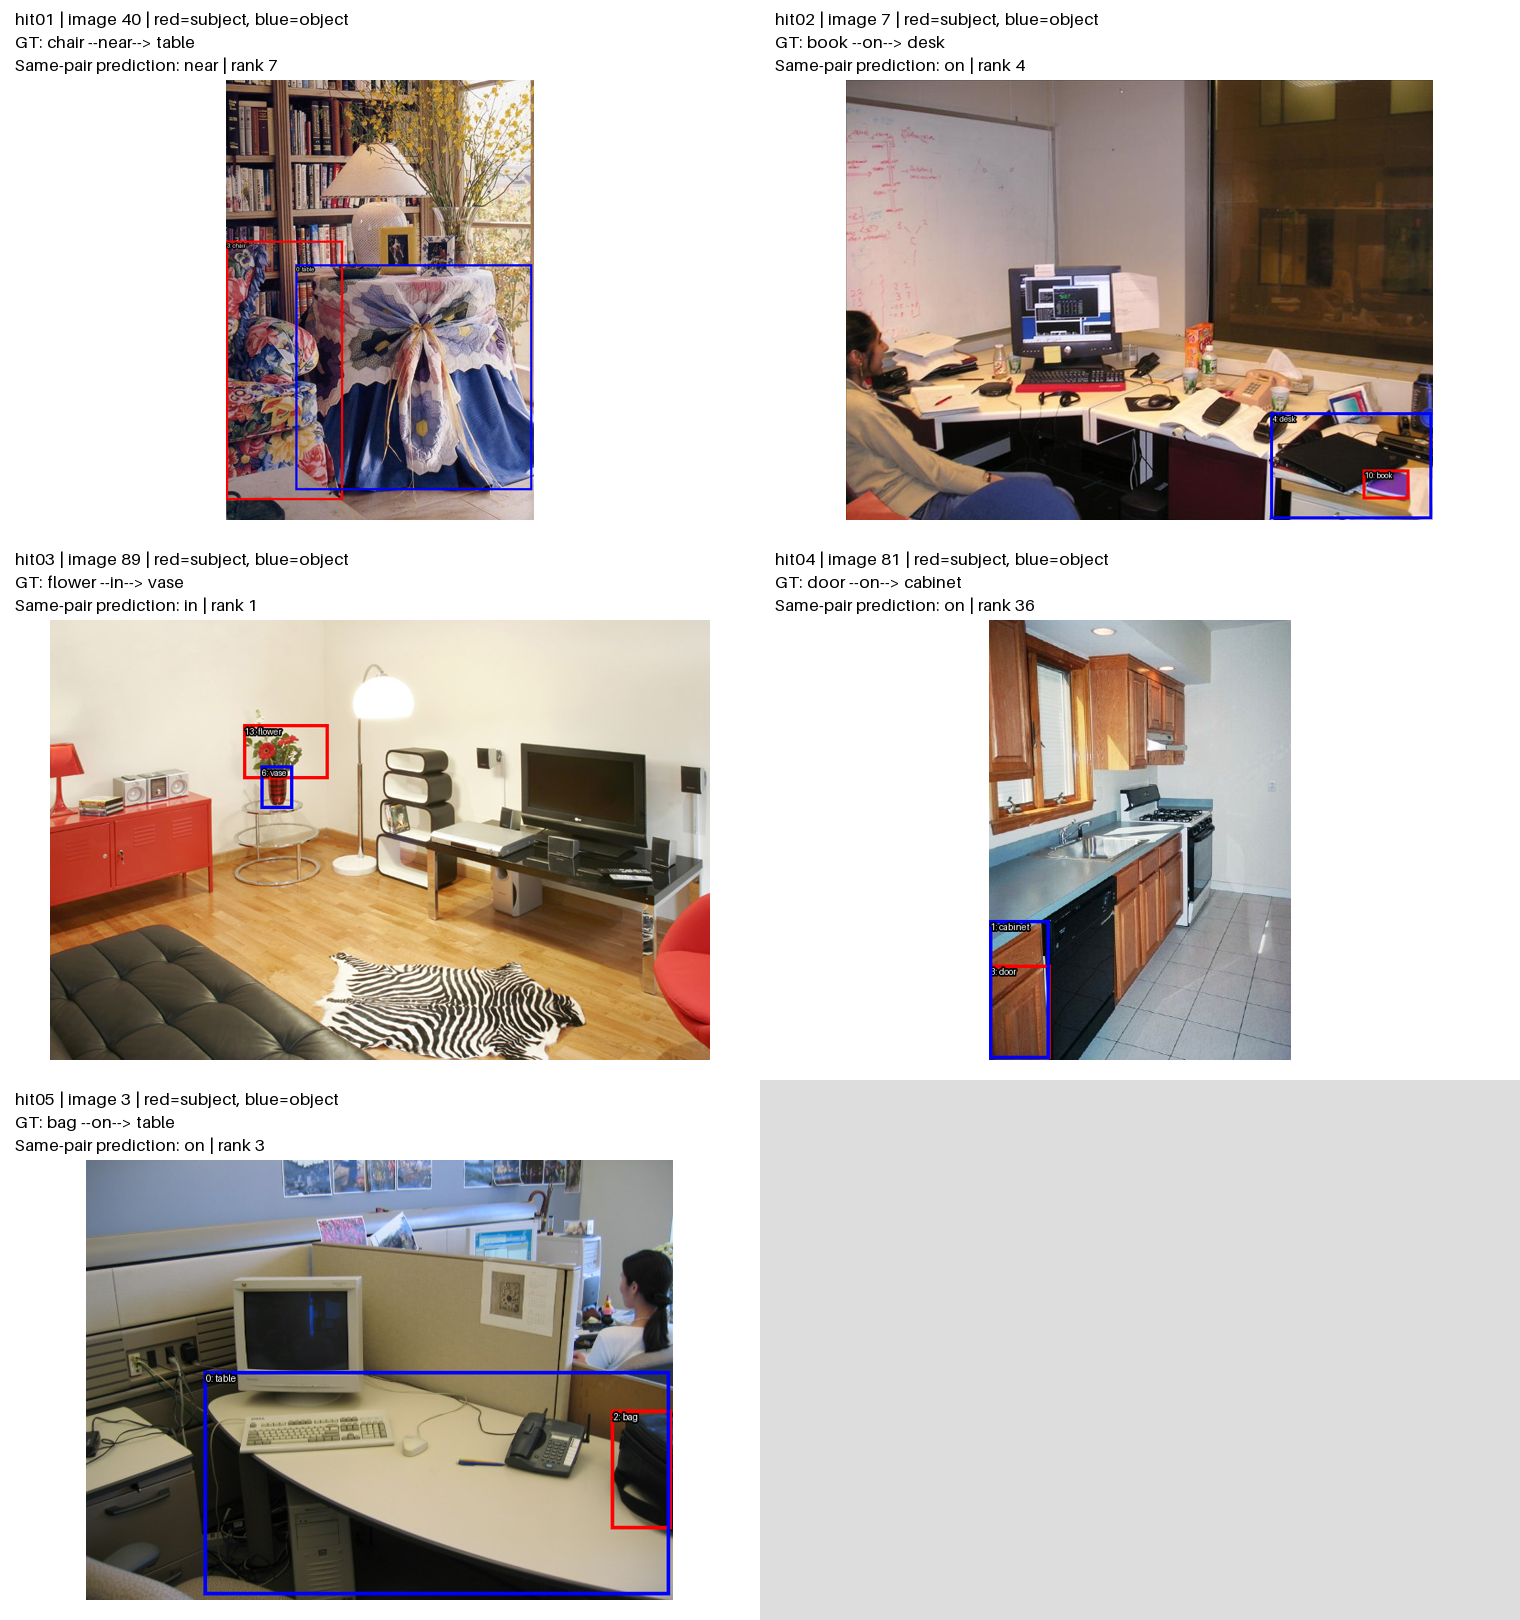
\includegraphics[width=.43\linewidth]{figures/vg-hit-contact-sheet.png}\hfill
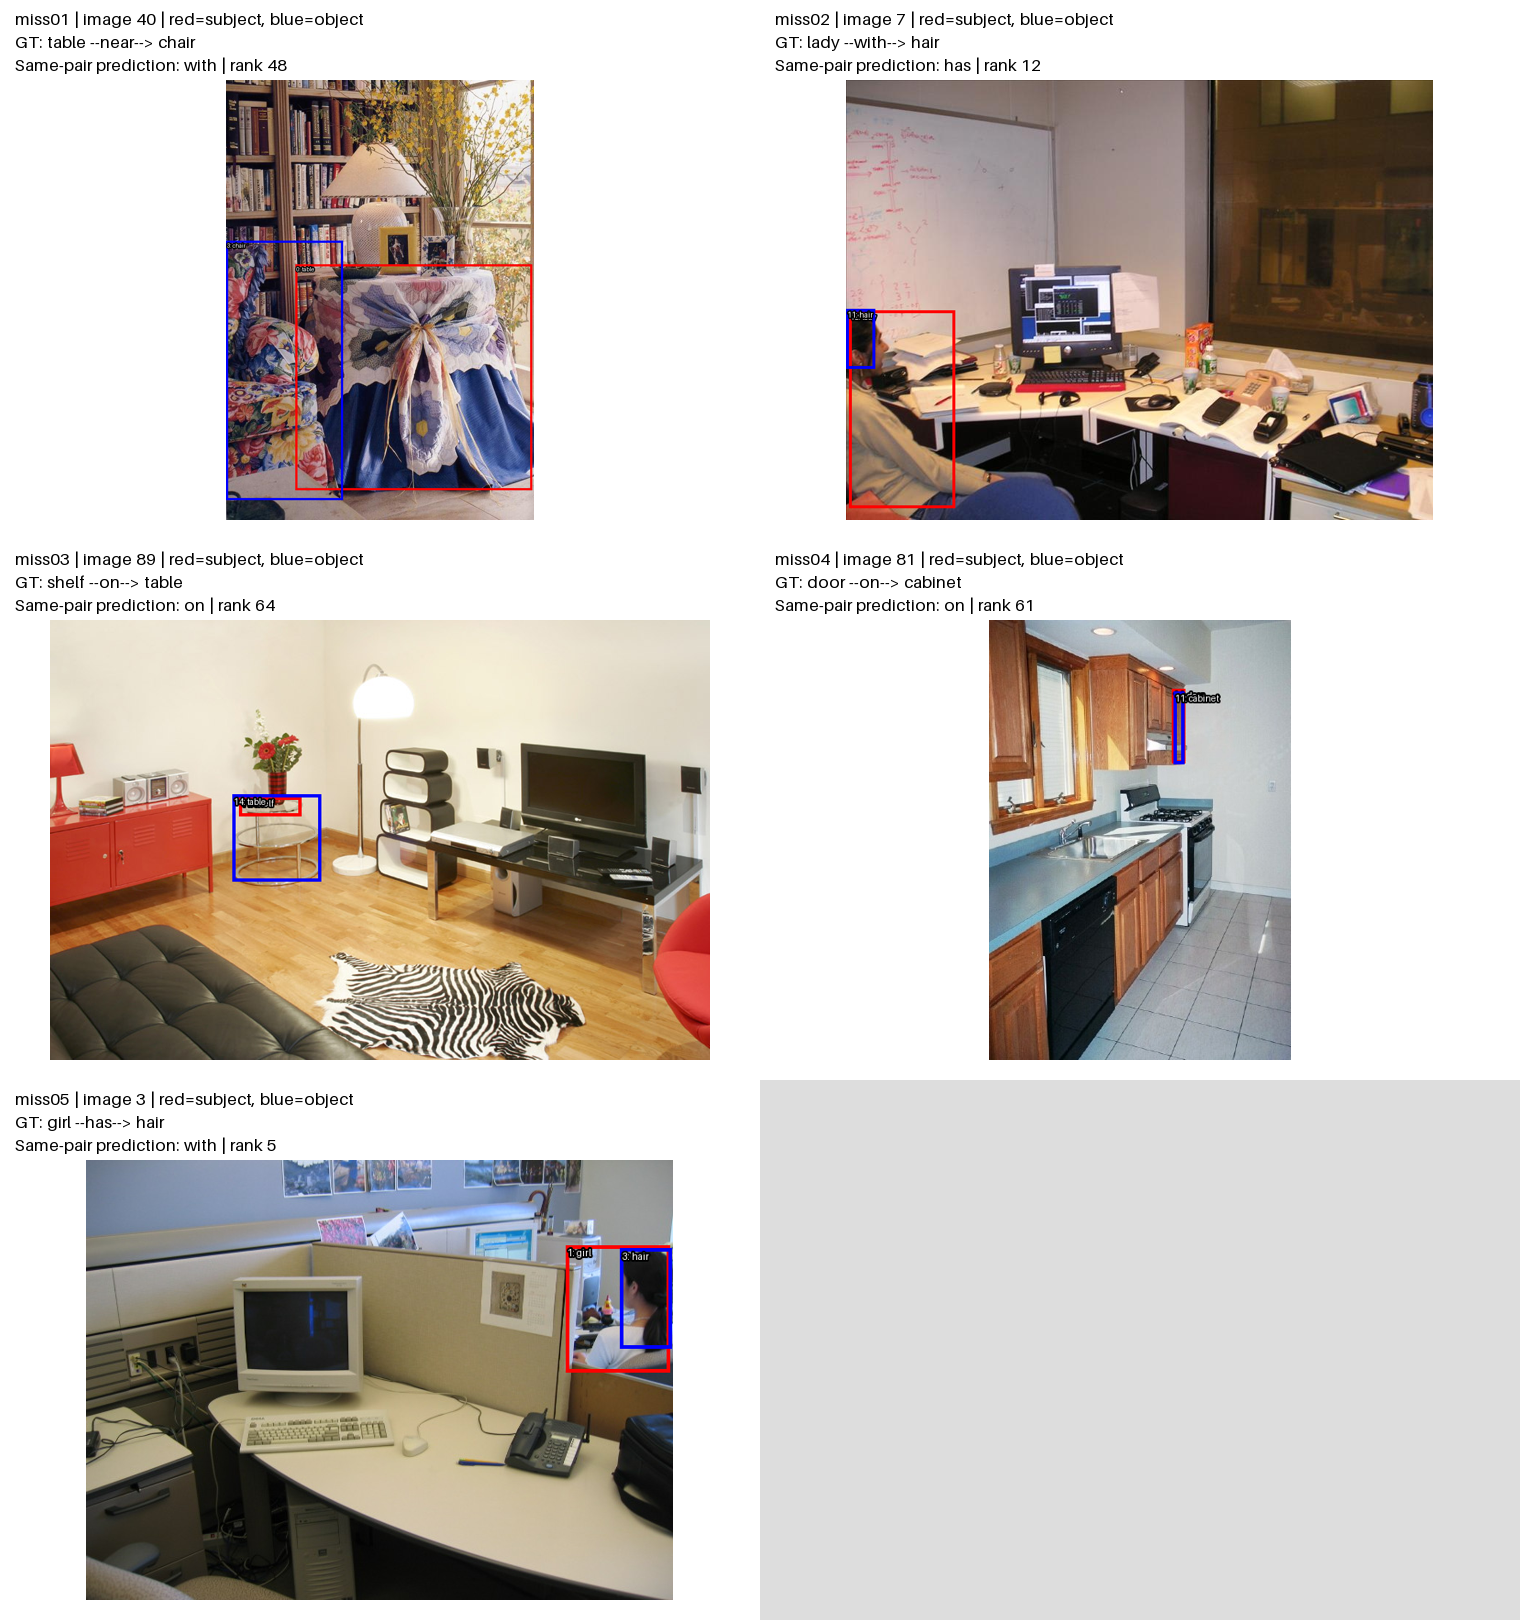
\includegraphics[width=.43\linewidth]{figures/vg-miss-contact-sheet.png}
\caption{Trái: H01--H05; phải: M01--M05, theo hàng từ trái sang phải.
Hộp đỏ là subject, xanh là object. Chi tiết GT và hạng nằm trong
bảng~\ref{tab:hits}--\ref{tab:misses}; ảnh gốc độ phân giải đầy đủ có trong artifact case.}
\end{figure}
\srcnote{Nguồn: \texttt{reports/level1/submission/cases/}.
Đây là case validation đã có, không gắn lại nhãn thành case test.}
